\chapter{\label{c:speedmeter-intro}The \SSMEXPT{}: introduction and technical design}

\section{Concept}
\begin{itemize}
  \item Usual literature review: use 2nd year report, Living Review, Graef et al, etc...
  \item Show Michelson response and noise. This should be radiation pressure dominated below the pole. Relate this to the analytical response equation I used in the controls paper for a Michelson.
  \item Introduce Sagnac speedmeter, showing it has better quantum noise IN ABSENCE OF ASYMMETRIES, and thus better overall sensitivity for equivalent shot noise. DON'T SHOW THE SSM SENSITIVITY HERE.
  \item Use Stefan D's labbook entry for response functions: p5648
  \item Introduce losses to show the degrading effect they have, introducing ``Michelson-like'' sensitivity. The main thing to show here is the effect on the quantum noise when there are asymmetries, like test mass asymmetry. This broadens the peak around the suspension resonance, which introduces the Michelson-like sensitivity.
  \item Mention significance of M8/M9/M10's reflectivity (c.f. loss) which can be expanded later in the controls chapter.
  \item See S.D.'s talk at group meeting 6th July, talking about how speed meters need a pi phase shift between photons hitting the same mirror to cancel R.P. noise. In a Sagnac it is naturally occurring but in a Michelson it requires a sloshing cavity or polarisation optics.
\end{itemize}

\subsection{\label{sec:position-meter-measurement}Sensitivity of a position-meter}
In an ordinary Michelson position-meter, the mirrors in each arm are sampled by separate light beams which recombine at the beam splitter. Motion of the mirror in the longitudinal direction either shortens or elongates the round-trip phase of the light in each arm, and thus this motion is imprinted upon the \emph{phase} of the light returning to the beam splitter. The phase difference of the two recombining beams at the beam splitter then leads to light at the output port, which can be measured using a heterodyne or homodyne readout as discussed in Section\,\ref{sec:readout}.

The presence of classical light power in the arms leads to a radiation pressure effect which imparts a force upon the test masses. A restoring force on the mirrors, either via a pendulum in a suspended experiment or a mirror mount on a table-top experiment, means that this force is static and the interferometer can be held at the operating point as discussed in Section\,\ref{sec:operating-point} by microscopic \gls{DC} corrections.

The responses of a simple Michelson interferometer and a Michelson interferometer with Fabry-Perot arm cavities are shown in Figure\,\ref{fig:mich-vs-fp-mich-response}. The change in light power at the output port is flat as a function of frequency at all frequencies in the \MI{}, and for the \FPMI{} it is flat up until the pole frequency of the \FP{} cavities, whereupon the response decreases due to the fact that mirror motion is no longer able to be witnessed by the light due to its finite travel time. The addition of arm cavities to the \MI{} results in greater response within the bandwidth of the cavities by a factor approximating the arm cavity finesse (see Appendix\,\ref{sec:cavity-fom}), in this case around \num{600}. Two other noticeable features occur, with the peak appearing at \SI{2}{\hertz} caused by an optical spring due to the detuning applied to the cavities for the purposes of \gls{DC} readout, and the trough at \SI{0.7}{\hertz} due to the mechanical pendulum resonance.

\begin{figure}
  \centering
  \includegraphics[width=\columnwidth]{graphics/generated/from-python/40-mich-vs-fp-mich-response.pdf}
  \caption[Response of a Michelson and Fabry-Perot Michelson]{\label{fig:mich-vs-fp-mich-response}Response of a \MI{} and a \FPMI{}. The \FPMI{} has arm cavities with finesse of around \num{600}, and so the response is increased by around this amount within the bandwidth of the cavities, which is around \SI{250}{\hertz}. The power at the output port has been matched in both cases by scaling the arm cavity detuning. The other features in the \FPMI{} are due to cavity mirror mechanics and optomechanics.}
\end{figure}

If we examine the quantum noise at the output of each interferometer, as shown in Figure\,\ref{fig:mich-vs-fp-mich-noise}, we see that the contribution from the \MI{} is white. This is \emph{quantum shot noise} as discussed in Section\,\ref{sec:quantum-shot-noise}, arising from quantum vacuum fluctuations. Without special techniques such as those discussed in Section\,\ref{sec:sub-sql-techniques}, this noise appears in the amplitude and phase of the light in equal proportions. In the \FPMI{} this flat noise still exists above around \SI{40}{\hertz}, but there also exists a low frequency slope proportional to $\frac{1}{f^2}$, for frequency $f$. This is \emph{quantum radiation pressure noise}, arising from the effect of the cavity mirrors' optomechanical conversion of fluctuations in amplitude into phase.

\begin{figure}
  \centering
  \includegraphics[width=\columnwidth]{graphics/generated/from-python/40-mich-vs-fp-mich-noise.pdf}
  \caption[Quantum noise of a Michelson and Fabry-Perot Michelson]{\label{fig:mich-vs-fp-mich-noise}Quantum noise at the output port of a \MI{} and a \FPMI{}.}
\end{figure}

If the mirrors were infinitely massive, no momentum would be imparted from the incident light and the light would then receive a phase change only from its round trip propagation, and the sensor would see only a noise contribution from shot noise. In the case of a physical mirror, there is some \emph{back-action} imparted by the amplitude of the incident light. Quantum shot noise contains amplitude fluctuations at all frequencies, and this is transformed by the effect of the mirror's mechanical susceptibility into motion due to the back-action force. A mechanical oscillator filters applied force to a greater extent at high frequencies, and so the conversion of amplitude into phase noise is in general a function of frequency and can be expressed in terms of the mirror's \emph{optomechanical coupling factor} $\kappa$ shown in Equation\,\ref{eq:optomechanicalcoupling} and plotted for the \FPMI{} discussed above in Figure\,\ref{fig:fp-mich-optomechanical-coupling}.

\begin{figure}
  \centering
  \includegraphics[width=\columnwidth]{graphics/generated/from-python/40-fp-mich-optomechanical-coupling.pdf}
  \caption[Optomechanical coupling factor for a \FPMI{}]{\label{fig:fp-mich-optomechanical-coupling}Optomechanical coupling factor for a \FPMI{} with \SI{40}{\kilo\gram} mirrors, \SI{1064e-9}{\nano\meter} laser light, \SI{20}{\kilo\watt} cavity power, arm length \SI{1}{\kilo\meter} and cavity half-bandwidth \SI{250}{\hertz}, calculated using Equation\,\ref{eq:optomechanicalcoupling}.}
\end{figure}

In a \FPMI{} with radiation pressure effects, the detector sees not only quantum shot noise but also quantum radiation pressure noise. These two effects combine to produce the quantum noise shown in Figure\,\ref{fig:mich-vs-fp-mich-noise}. The quantum noise limited sensitivity of the interferometer is given by the ratio of the quantum noise at the sensor to the response of the interferometer to that sensor, and so for differential arm cavity motion it is simply the ratio of the curves in Figures \ref{fig:mich-vs-fp-mich-noise} and \ref{fig:mich-vs-fp-mich-response}, shown in Figure\,\ref{fig:mich-vs-fp-mich-sensitivity}. By scaling the mass and laser power it is possible to set the frequency cut-off above and below which the quantum shot noise and quantum radiation pressure noise sources dominate, but as shown in Section\,\ref{sec:sql} the combination of these two sources of quantum noise creates a fundamental limit to the sensitivity of position meters known as the \gls{SQL}.

\begin{figure}
  \centering
  \includegraphics[width=\columnwidth]{graphics/generated/from-python/40-mich-vs-fp-mich-sensitivity.pdf}
  \caption[Quantum noise limited sensitivity of a Michelson and Fabry-Perot Michelson]{\label{fig:mich-vs-fp-mich-sensitivity}Quantum noise limited sensitivity of a \MI{} and a \FPMI{}.}
\end{figure}

\subsection{\label{sec:speed-meter-measurement}Sensitivity of a speed-meter}
Since the early 1990s it has been known that the measurement of momentum, known to be a quantum non-demolition (\gls{QND}) observable, offers the ability to surpass the \gls{SQL} in interferometric measurement \cite{Braginsky1990}. Initial suggestions for the conversion of an interferometer into a speed-meter involved the Michelson topology, for instance with the addition of a \emph{sloshing cavity} \cite{Braginsky2000, Purdue2002} at the output port, as shown in Figure\,\ref{fig:sloshing-michelson}.

\begin{figure}
  \centering
  \includegraphics[width=\columnwidth]{graphics/generated/from-svg/40-sloshing-michelson.pdf}
  \caption[Layout of a \MI{} with a sloshing cavity]{\label{fig:sloshing-michelson}Layout of a \MI{} with a sloshing cavity as presented in \cite{Purdue2002}. The light leaving the standard \MI{} is coupled into a sloshing cavity via a beam splitter where it receives a phase shift, and it re-enters the interferometer via the recycling mirror to the left of the sloshing beam splitter. The light incident upon the beam splitter then contains light that has sampled the mirrors at two points in time, leading to a speed-meter effect.}
\end{figure}

It was realised by Chen \cite{Chen2003} that the zero-area \SSM{} is a speed-meter. This topology is arranged such that incident photons sample the same set of mirrors in two directions at two different times, leading to the speed-meter behaviour shown in Equation XXX...

\section{The \SSMEXPT{}}
The method on which we focus employs an interferometer topology intrinsically sensitive to a \gls{QND} observable \cite{Danilishin2012}. The measurement of velocity, itself approximately proportional to the \gls{QND} observable of the free test mass momentum, is one way in which a reduction in quantum radiation pressure noise can be achieved. A proof-of-concept experiment is under way at the University of Glasgow to demonstrate an audio-band reduction of quantum radiation pressure noise in a \SSM{} topology over an equivalent Michelson design \cite{Graef2014}. This topology is being considered as an alternative to the \ET{}'s \MI{} design \cite{MuellerEbhardt2009a, Voronchev2015}. The topology under investigation in the proof-of-concept experiment utilises a zero-area Sagnac interferometer with the addition of arm cavities based on the concept presented in ref.\,\cite{Chen2003}. By design, this interferometer produces a signal at the beam splitter's output port proportional to differential arm cavity mirror \emph{velocity}, in contrast to the \emph{displacement}-proportional signal sensed in the Michelson topology.

\subsection{Loss in \SSM{}s}
\note{Change in slope of sensitivity in speedmeter at low frequencies. This is due to an imbalanced beam splitter and is described in Stefan Danilishin's asymmetries paper at the end of section 2.5. It shows mathematically why this happens.}

\subsection{\label{sec:bhd-intro}Balanced homodyne detection}
\note{Explain homodyne angle, basic description.}

\section{Implementation}

Some technical challenges in the implementation of the speedmeter are discussed in this chapter. Certain topics involve substantially more scientific endeavour and are thus presented as discrete chapters: the control of the primary degree of freedom of the speedmeter, presented in Chapter X; and a proof-of-principle experiment to demonstrate a new type of actuator, presented in Chapter Y.

\subsection{Experimental design}
\note{Discuss the experiment layout, power, cavity lengths, etc. Introduce the real sensitivity curves here.}

\subsection{Mechanics}
\note{Vacuum system requirements, tanks, optical table, suspensions, seismic noise, etc.}

\subsection{Layout}

\begin{figure}
  \centering
  \includegraphics[width=\columnwidth]{graphics/generated/from-svg/40-speedmeter-layout.pdf}
  \caption[\SSMEXPT{} layout]{\label{fig:ssm-layout}\SSMEXPT{} layout.}
\end{figure}

\subsection{Sensing and control}

\subsubsection{Longitudinal control}

\subsubsection{Lock acquisition}
\note{See Andreas' thesis}

\subsubsection{Angular control}

\subsubsection{Frequency stabilisation}

\subsubsection{\label{sec:cds}CDS data acquisition system}

\note{Introduce CDS with the Bork reference, as it is required for Chapters 5 and 7}

\subsubsection{Avoidance of ground loops}

One of the main issues faced by experiments involving numerous interfaces between digital and analogue devices is the creation of ground loops. Effectively an antenna.

\note{Avoidance of ground loops, interfacing with CDS, in-vacuum wiring: why it needs careful thought, etc}
\note{Display wiring diagrams in landscape mode, full page}

\note{Generate A4 versions of wiring diagrams for inclusion here.}

\subsubsection{Connectors}
\note{How we avoided plugging the wrong things in, i.e. why we use DB9/DB15/DB25 etc.}
\note{Differential sending - take stuff from HV chapter on CMRR?}

\subsubsection{In-vacuum signalling}
\note{Octopus cables, strain relief housing, etc.}

\begin{figure}
  \centering
  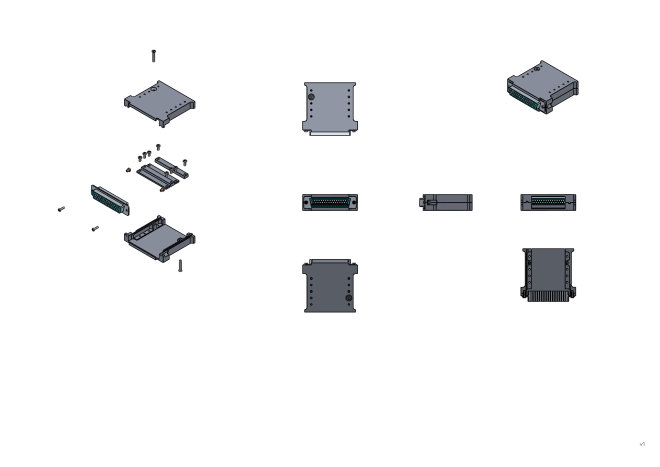
\includegraphics[width=0.75\columnwidth]{graphics/40-db50-housing.png}
  \caption[In-vacuum DB50 octopus cable housing]{In-vacuum DB50 housing for octopus cable.}
  \label{fig:db50-housing}
\end{figure}

\subsubsection{Auxiliary coil drivers}
\note{Put aux coil driver stuff here}
\note{Auxiliary coil driver subrack wiring design / motivation / assembly}
\note{Backplane board design - talk about rationale, show Eagle diagrams, etc.}

\begin{figure}
  \centering
  \includegraphics[width=\columnwidth]{graphics/generated/from-svg/40-auxiliary-octopus-cable.pdf}
  \caption[Auxiliary octopus cable schematic]{\label{fig:aux-octopus-cable-wiring}``Octopus'' cable for breaking out a DB50 connector into DB9 connectors to allow signals to be sent to each of the coils on seven auxiliary suspensions.}
\end{figure}

\begin{figure}
  \centering
  \includegraphics[width=\columnwidth]{graphics/generated/from-svg/40-auxiliary-suspension.pdf}
  \caption[Auxiliary suspension coil schematic]{\label{fig:aux-suspension-wiring}Auxiliary suspension coil schematic.}
\end{figure}

\begin{figure}
  \centering
  \includegraphics[width=\columnwidth]{graphics/generated/from-svg/40-auxiliary-backplane-board.pdf}
  \caption[Auxiliary subrack backplane board schematic]{\label{fig:aux-backplane-schematic}Auxiliary coil driver subrack backplane. Auxiliary coil driver cards can be plugged in to this board, which then maps the signals to a DB50 connector which connects to the vacuum feedthrough. This routes four coil signals (five conductors including ground) per coil driver, for seven coil drivers, to one DB50 connector. This can then be connected to the vacuum system, where the auxiliary octopus cable (see Figure XXX) maps these signals to individual auxiliary suspensions.}
\end{figure}

\begin{figure}
  \centering
  \includegraphics[width=\columnwidth]{graphics/generated/from-svg/40-auxiliary-backplane-interface.pdf}
  \caption[Auxiliary subrack backplane interface]{\label{fig:aux-backplane-interface}Auxiliary coil driver subrack backplane interface.}
\end{figure}

\section{Modelling the sensitivity of the \SSM{}}
\note{Optickle and Finesse models, analytical comparison}

\section{Topics of particular focus}
\note{Introduce the work to be discussed in the controls and ESD chapters.}

\subsection{Control and noise analysis of the Glasgow \SSM{}}

\subsection{Demonstration of a plate-capacitor electrostatic actuator}